\documentclass[11pt]{article}
\usepackage[a4paper,margin=1in]{geometry}
\usepackage{amsmath,amssymb,mathtools,bm}
\usepackage{hyperref}
\usepackage{tikz}
\usetikzlibrary{calc,decorations.pathreplacing}

\newcommand{\al}{\alpha'}
\newcommand{\perpD}{D_\perp}
\newcommand{\RR}{\mathbb{R}}
\newcommand{\ZZ}{\mathbb{Z}}
\newcommand{\ii}{\mathrm{i}}
\newcommand{\dd}{\mathrm{d}}
\newcommand{\arxiv}[1]{\href{https://arxiv.org/abs/#1}{arXiv:#1}}
\newcommand{\doi}[1]{\href{https://doi.org/#1}{doi:#1}}

\title{Lightcone Mandelstam Amplitudes with Discrete \texorpdfstring{$\sigma$}{sigma}}
\author{}
\date{\today}

\begin{document}
\maketitle

\section{Goal}
We want a practical formulation of lightcone bosonic and superstring amplitudes in Mandelstam parametrization where:
\begin{itemize}
\item the worldsheet spatial direction $\sigma$ is discretized,
\item each propagator cylinder is an exactly solvable Gaussian (free transverse bosons $X^i$ and free GS fermions $\theta^\alpha$),
\item the kinematic overlap of full string boundaries is imposed exactly, leaving only a local interaction-point prefactor as the nontrivial dynamical input.
\end{itemize}

The main output should be a computable expression for amplitudes in which all bulk integrations are already done analytically.

\section{What is standard vs what is new}
Most structural ingredients are classical:
\begin{itemize}
\item Mandelstam lightcone diagrams and parametrization,
\item Green--Schwarz lightcone free worldsheet fields,
\item interaction-point insertions required by supersymmetry/Lorentz symmetry.
\end{itemize}
The key step here is different in emphasis: discretize only the worldsheet spatial coordinate $\sigma$ so that, at any loop order, each propagator becomes a finite-dimensional Gaussian kernel that is exactly computable. This turns the higher-loop problem into a controlled numerical task:
\begin{equation}
\begin{aligned}
{\cal A}_{h\text{-loop}}
=\int \dd\mu_{\text{moduli}}\;
{\cal G}_{\text{free}}(N,T)\;
{\cal I}_{\text{int}}(N,T).
\end{aligned}
\end{equation}

\section{Literature status}
A first literature pass suggests that the basic interaction-point problem is indeed old, but the discrete-$\sigma$ numerical version is not already sitting on the shelf in the form we need.

First, the lightcone Green--Schwarz construction of string interactions is classical. Green and Schwarz already constructed lightcone vertex operators for superstrings in their early work and then wrote down an off-shell three-string interaction vertex together with the cubic correction to the supercharge in \cite{GreenSchwarz1982Vertices,GreenSchwarz1983Interactions}. Green and Seiberg later emphasized that cubic overlap data alone is not the full story: contact interactions are required in lightcone gauge \cite{GreenSeiberg1988}.

Second, the interaction-point operator itself was recognized as the awkward part of the Green--Schwarz formalism. Berkovits explicitly stresses that lightcone and semi-lightcone Green--Schwarz amplitudes are complicated by non-trivial interaction-point operators, and shows that alternative super-worldsheet/twistor formulations can eliminate them \cite{Berkovits1992N20,Berkovits1993Twistor}.

Third, the continuum Green--Schwarz interaction-point prefactor is known explicitly. In the pp-wave literature, Spradlin and Volovich give the SO$(8)$-covariant octic polynomial $v_{IJ}(\Lambda)$, and Pankiewicz and Stefanski write the full dressed cubic vertex with the bosonic interaction-point operators $K^I,\widetilde K^J$ \cite{SpradlinVolovich2002,PankiewiczStefanski2002}. In flat space, these are the structures one should recover in the appropriate limit.

Fourth, there is a closely related matrix-string line of thought. Dijkgraaf, Verlinde and Verlinde identify perturbative string interactions in the matrix-string framework \cite{DVV1997Matrix}. Dijkgraaf and Motl then relate the Green--Schwarz lightcone interaction Hamiltonian to the twist-field formalism and analyze higher-order contact terms \cite{DijkgraafMotl2003}. Kishimoto, Moriyama and Teraguchi make the relation between matrix-string twist fields and the lightcone three-string vertex even more explicit \cite{Kishimoto2006}. More recently, Ando, Fujii, Kunitomo and Totsuka-Yoshinaka show that collisions of local operators remain a central issue in constructing a consistent lightcone-gauge superstring field theory \cite{Ando2025}.

The conclusion I draw from these papers is the following. The continuum cubic prefactor is not the unknown part; it is already fixed by dynamical supersymmetry. The new step in this note is to rewrite the full problem in a discrete-$\sigma$ language where the propagators are exact Gaussians, the boundary overlap is imposed directly in position space, and the known continuum prefactor is discretized into a local operator at the join. Contact terms at order $g^2$ are still expected, as already emphasized in \cite{GreenSeiberg1988,GreensiteKlinkhamer1988}.

\section{Mandelstam map and lightcone time}
For a fixed lightcone diagram (tree or loop), use Mandelstam's map
\begin{equation}
\rho(z)=\sum_{r=1}^{n}\alpha_r^{\mathrm{M}} \log(z-Z_r),\qquad \sum_{r=1}^n \alpha_r^{\mathrm{M}}=0,\qquad \alpha_r^{\mathrm{M}}=2\al p_r^+\times(\text{in/out sign}).
\end{equation}
After Wick rotation to Euclidean worldsheet time, we use the convention $\tau=\Re \rho$ and $\sigma=\Im \rho$.
External legs are semi-infinite cylinders of circumference $|\alpha_r^{\mathrm{M}}|$.
Internal propagators are finite cylinders with Schwinger lengths $T_e$ given by differences of $\tau$-coordinates between neighboring interaction points. For loop diagrams, one must also keep the relative translation in $\sigma$ used to glue the two ends of a propagator. Thus the propagator data are $(T_e,\varphi_e)$ rather than just $T_e$, where $\varphi_e$ is the twist modulus along the $\sigma$ circle.

In the discrete lattice formulas below I use the positive cylinder circumferences
\begin{equation}
\alpha_r \equiv |\alpha_r^{\mathrm{M}}|,
\end{equation}
and keep the orientation signs separately through factors such as $\epsilon_r=(+1,+1,-1)$ in the canonical one-form. Thus for a cubic join with two incoming legs $1,2$ and one outgoing leg $3$, the signed Mandelstam residues obey $\alpha_1^{\mathrm{M}}+\alpha_2^{\mathrm{M}}+\alpha_3^{\mathrm{M}}=0$, while the positive circumferences satisfy $\alpha_3=\alpha_1+\alpha_2$ and hence $N_3=N_1+N_2$.

For a discrete $\sigma$ lattice, string $r$ has $N_r$ sites with
\begin{equation}
a_r=\frac{\alpha_r}{N_r},\qquad \sigma_n=n\,a_r,\quad n=0,\dots,N_r-1.
\end{equation}
At a cubic join, $p_3^+=p_1^++p_2^+$ implies
\begin{equation}
N_3=N_1+N_2,
\end{equation}
after choosing a common lattice spacing (or an integer-compatible refinement).

The basic propagator building block is shown in Figure~\ref{fig:discrete-cylinder}.

\begin{figure}[t]
\centering
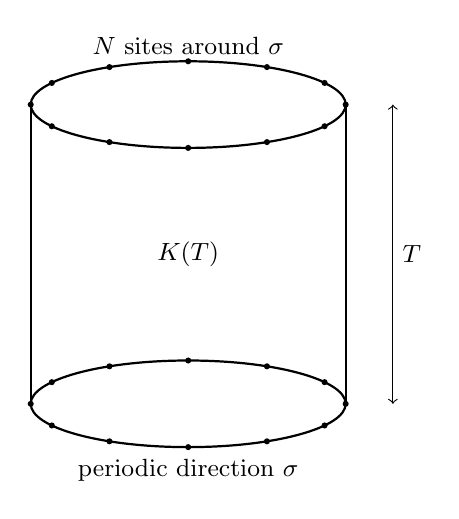
\begin{tikzpicture}[scale=1.0, every node/.style={font=\small}]
\draw[thick] (0,0) ellipse (2 and 0.55);
\draw[thick] (0,3.8) ellipse (2 and 0.55);
\draw[thick] (-2,0) -- (-2,3.8);
\draw[thick] (2,0) -- (2,3.8);
\foreach \ang in {0,30,...,330} {
  \fill ({2*cos(\ang)},{0.55*sin(\ang)}) circle (1.1pt);
  \fill ({2*cos(\ang)},{3.8 + 0.55*sin(\ang)}) circle (1.1pt);
}
\draw[<->] (2.6,0) -- node[right] {$T$} (2.6,3.8);
\node at (0,4.55) {$N$ sites around $\sigma$};
\node at (0,1.9) {$K(T)$};
\node at (0,-0.85) {periodic direction $\sigma$};
\end{tikzpicture}
\caption{A propagator cylinder in the discrete-$\sigma$ scheme. Only the spatial direction is discretized; Euclidean lightcone time $\tau$ remains continuous. The resulting propagator is an exact finite-dimensional Gaussian kernel.}
\label{fig:discrete-cylinder}
\end{figure}

\section{Discrete free boson on a cylinder}
For one transverse coordinate on a cylinder of length $T$ and $N$ sites:
\begin{equation}
S_B=\frac{1}{4\pi\al}\int_0^T\dd\tau\sum_{n=0}^{N-1}
\left[a\,(\partial_\tau X_n)^2+\frac{1}{a}(X_{n+1}-X_n)^2\right],\qquad X_N\equiv X_0.
\end{equation}
Fourier modes
\begin{equation}
X_n(\tau)=\frac{1}{\sqrt{N}}\sum_{k=0}^{N-1}q_k(\tau)e^{2\pi \ii kn/N},
\end{equation}
diagonalize the action with frequencies
\begin{equation}
\omega_k=\frac{2}{a}\sin\left(\frac{\pi k}{N}\right),\qquad k=0,\dots,N-1.
\end{equation}
For $k\neq 0$ (Euclidean harmonic oscillator),
\begin{equation}
K_{B,k}(q_f,q_i;T)=
\left(\frac{m\omega_k}{2\pi\sinh(\omega_k T)}\right)^{1/2}
\exp\!\left[
-\frac{m\omega_k}{2\sinh(\omega_k T)}
\big((q_f^2+q_i^2)\cosh(\omega_k T)-2q_fq_i\big)
\right],
\end{equation}
with
\begin{equation}
m=\frac{a}{2\pi\al}.
\end{equation}
This displayed formula is the kernel for one independent \emph{real} oscillator degree of freedom. Equivalently, it applies to the independent half-spectrum or to the real and imaginary parts of a nonzero Fourier mode. If instead one keeps the full complex mode $q_k$ together with the reality condition $q_{N-k}=\bar q_k$, then the pair $(k,N-k)$ contributes
\begin{equation}
K_{B,k}^{\mathrm{cx}}(q_f,q_i;T)=
\frac{m\omega_k}{2\pi\sinh(\omega_k T)}
\exp\!\left[
-\frac{m\omega_k}{2\sinh(\omega_k T)}
\left(
\bigl(|q_f|^2+|q_i|^2\bigr)\cosh(\omega_k T)
-2\Re(\bar q_f q_i)
\right)
\right],
\end{equation}
with unit power in the prefactor because the complex mode carries two real degrees of freedom. The site-basis Gaussian matrices below avoid this bookkeeping issue by working directly in the full real position space.
For $k=0$ (free particle),
\begin{equation}
K_{B,0}(q_f,q_i;T)=
\left(\frac{m}{2\pi T}\right)^{1/2}
\exp\!\left[-\frac{m(q_f-q_i)^2}{2T}\right].
\end{equation}
The full bosonic cylinder kernel is the product over modes and transverse directions $i=1,\dots,\perpD$.

For loop propagation one must also include a twist in $\sigma$. If $\varphi\in[0,1)$ denotes the fraction of the circumference by which one end of the cylinder is shifted relative to the other, then
\begin{equation}
X_f(\sigma)=X_i(\sigma+\varphi |\alpha|).
\end{equation}
On the lattice this is implemented by a shift operator $R_N(\varphi)$ acting in $\sigma$ position space. For an exact lattice shift $\varphi N\in \ZZ$,
\begin{equation}
\bigl(R_N(\varphi)X\bigr)_n = X_{n+\varphi N \,\, \mathrm{mod}\,N},
\end{equation}
while for general $\varphi$ one defines the same operator spectrally by
\begin{equation}
R_N(\varphi)=F^\dagger \, \mathrm{diag}\!\left(e^{2\pi \ii k\varphi}\right) F.
\end{equation}
The twisted bosonic propagator is then
\begin{equation}
K_B(X_f,X_i;T,\varphi)=K_B\bigl(X_f,R_N(\varphi)X_i;T,0\bigr),
\end{equation}
so each discrete Fourier mode picks up the phase $e^{2\pi \ii k\varphi}$ in the cross-term.

\section{Discrete free GS fermions on a cylinder}
In lightcone GS gauge, the transverse fermions are free. After Fourier transform in $\sigma$, each mode gives a quadratic Grassmann system. A convenient bookkeeping device is to complexify the eight real GS spinor components and use coherent-state labels $\eta_{k,a}$, $\bar\eta_{k,a}$ with $a=1,\dots,8$. This is only a representation choice, not a physical doubling; the equivalent real Majorana formulation and its Pfaffian appear below. In these variables one can write
\begin{equation}
S_F=\int_0^T\dd\tau\sum_{k,a}\bar\eta_{k,a}(\partial_\tau+\omega_k)\eta_{k,a},
\end{equation}
where $a$ labels GS spinor components (and similarly for right movers). The same lattice frequencies $\omega_k$ appear as in the bosonic sector because the lightcone GS worldsheet theory is free with matched transverse mode spectrum, even though worldsheet supersymmetry is not manifest.
Hence each nonzero mode has exact kernel
\begin{equation}
K_{F,k}(\bar\eta_f,\eta_i;T)=
\exp\!\left[\bar\eta_f\,e^{-\omega_k T}\eta_i\right],
\end{equation}
up to convention-dependent normalization factors that can be fixed once and for all from vacuum-to-vacuum propagation.
For the zero mode one has $\omega_0=0$ and therefore
\begin{equation}
K_{F,0}(\bar\eta_f,\eta_i;T)=
\exp\!\left[\bar\eta_f\,\eta_i\right],
\end{equation}
independent of $T$. This is the cylinder transport of the GS fermionic zero mode and is the finite-$N$ precursor of the local Grassmann data later organized into $\Lambda^a$.

With a geometric twist in $\sigma$, the fermionic cross-term acquires the same phase,
\begin{equation}
K_{F,k}(\bar\eta_f,\eta_i;T,\varphi)=
\exp\!\left[\bar\eta_f\,e^{-\omega_k T}e^{2\pi \ii k\varphi}\eta_i\right],
\end{equation}
up to additional sign choices associated with the fermionic spin structure around the loop.

So both bosonic and fermionic propagators are exactly computable Gaussians on the discrete cylinder, with dependence on both $T$ and the $\sigma$-twist $\varphi$.

\section{Explicit site-basis Gaussian matrices}
For numerical assembly, it is best to keep each cylinder kernel in the form
\begin{equation}
K_B(X_f,X_i;T,\varphi)=
{\cal N}_B(T)\,
\exp\!\left[
-\frac12 X_f^{\!T}A(T)X_f
-\frac12 X_i^{\!T}A(T)X_i
+X_f^{\!T}B(T,\varphi)X_i
\right].
\end{equation}
Let $\mu \equiv a/(2\pi\al)$ and let $F$ be the unitary DFT matrix on $N$ sites. Then
\begin{align}
A(T)&=\mu\,F^\dagger\,
\mathrm{diag}\!\big(\omega_k\coth(\omega_k T)\big)\,F,\\
B(T,\varphi)&=\mu\,F^\dagger\,
\mathrm{diag}\!\big(e^{2\pi \ii k\varphi}\omega_k\mathrm{csch}(\omega_k T)\big)\,F.
\end{align}
For the zero mode, use the smooth limits
\begin{equation}
\omega_0\coth(\omega_0 T)\to \frac{1}{T},\qquad
\omega_0\mathrm{csch}(\omega_0 T)\to \frac{1}{T}.
\end{equation}
Hence $A(T)$ is circulant in site space, while $B(T,\varphi)$ is a twisted circulant matrix. Both are diagonalized exactly by the same DFT.

For fermions (coherent states),
\begin{equation}
K_F(\bar\eta_f,\eta_i;T,\varphi)=
{\cal N}_F(T)\,
\exp\!\left[\bar\eta_f^{\!T}U(T,\varphi)\eta_i\right],\qquad
U(T,\varphi)=F^\dagger\mathrm{diag}\!\big(e^{-\omega_k T}e^{2\pi \ii k\varphi}\big)F.
\end{equation}
The $k=0$ entry of $U(T,\varphi)$ is exactly $1$, so the fermionic zero mode propagates without any $T$-dependent damping.

These formulas are the core building blocks for every edge in a higher-loop diagram. At higher genus the independent twist moduli are integrated together with the Schwinger lengths.

Figure~\ref{fig:twisted-cylinder} shows the geometric meaning of the twist modulus in $\sigma$ position space.

\begin{figure}[t]
\centering
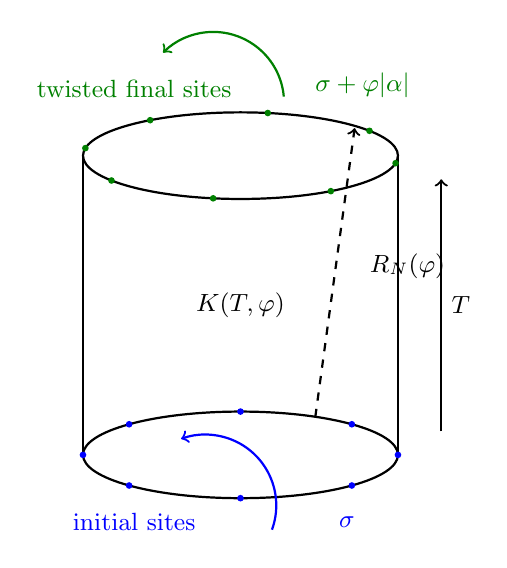
\begin{tikzpicture}[scale=1.0, every node/.style={font=\small}]
\draw[thick] (0,0) ellipse (2 and 0.55);
\draw[thick] (0,3.8) ellipse (2 and 0.55);
\draw[thick] (-2,0) -- (-2,3.8);
\draw[thick] (2,0) -- (2,3.8);
\foreach \ang in {0,45,...,315} {
  \fill[blue] ({2*cos(\ang)},{0.55*sin(\ang)}) circle (1.2pt);
}
\foreach \ang in {35,80,...,350} {
  \fill[green!50!black] ({2*cos(\ang)},{3.8 + 0.55*sin(\ang)}) circle (1.2pt);
}
\draw[->,thick] (2.55,0.3) -- node[right] {$T$} (2.55,3.5);
\draw[->,thick,blue] (0.4,-0.95) arc[start angle=-20,end angle=110,radius=0.9];
\node[blue] at (1.35,-0.85) {$\sigma$};
\draw[->,thick,green!50!black] (0.55,4.55) arc[start angle=5,end angle=135,radius=0.9];
\node[green!50!black] at (1.55,4.7) {$\sigma+\varphi|\alpha|$};
\draw[->,dashed,thick] (0.95,0.48) -- (1.45,4.15);
\node[right] at (1.52,2.4) {$R_N(\varphi)$};
\node at (0,1.9) {$K(T,\varphi)$};
\node[blue] at (-1.35,-0.85) {initial sites};
\node[green!50!black] at (-1.35,4.65) {twisted final sites};
\end{tikzpicture}
\caption{Twisted propagator cylinder. The lower circle is glued to the upper circle after a translation by $\varphi|\alpha|$ along the $\sigma$ direction. In Fourier space this becomes multiplication by the phase $e^{2\pi \mathrm{i}k\varphi}$; in site space it is the shift operator $R_N(\varphi)$.}
\label{fig:twisted-cylinder}
\end{figure}

\section{Sewing formula for a fixed diagram}
For a diagram ${\cal D}$ with internal edges $e$ and cubic vertices $I$:
\begin{equation}
{\cal A}_{\cal D}=
\int\prod_e \dd T_e
\int\prod_A \dd\varphi_A\;
J_{\mathrm{M}}(T,\varphi;\alpha_{\mathrm{ext}})
\int\prod_{\text{internal boundaries}}\dd X\,\dd\Theta\;
\prod_e K_e(X_f,\Theta_f;X_i,\Theta_i;T_e,\varphi_e)\,
\prod_I {\cal V}_I.
\end{equation}
Choose a basis of graph cycles $A=1,\dots,h$. Then only $h$ twists are independent, and the twist carried by an individual internal edge is
\begin{equation}
\varphi_e=\sum_{A=1}^{h}\epsilon_{eA}\varphi_A
\qquad
(\mathrm{mod}\,1),
\end{equation}
with incidence numbers $\epsilon_{eA}\in\{0,\pm1\}$ determined by how edge $e$ winds around the chosen homology basis. The vertex overlap constrains all other relative $\sigma$ shifts.
All nonlocal dependence on worldsheet geometry/moduli sits in $K_e$ through $T_e$, $\varphi_e$, and $N_e$. Since each $K_e$ is explicit, the unresolved ingredient is the local vertex factor ${\cal V}_I$.

For actual amplitudes this lightcone measure must be multiplied by the Mandelstam/Jacobian factor relating the Schwinger-twist parameters to the true moduli of the punctured Riemann surface:
\begin{equation}
\dd\mu_{\mathrm{lc}}
=
J_{\mathrm{M}}(T,\varphi;\alpha_{\mathrm{ext}})
\prod_e \dd T_e
\prod_A \dd\varphi_A.
\end{equation}
At tree level $J_{\mathrm{M}}$ is the usual Jacobian between interaction times and Koba--Nielsen data; at loop level it is the determinant relating the lightcone parameters to Teichmuller moduli. This factor is independent of the finite-dimensional Gaussian sewing and should be included as part of the final moduli measure.

External states are inserted as boundary wavefunctionals $\Psi_r[X_{\mathrm{ext}}^{(r)},\Theta_{\mathrm{ext}}^{(r)}]$ on the semi-infinite external cylinders. Equivalently, one may attach cylinders of finite length $T_{\mathrm{ext}}$ and then take $T_{\mathrm{ext}}\to\infty$ to project onto the chosen external Fock states. At tree level there is no independent twist integral, so closed-string level matching of the external states must be imposed by this external-state projection. At loop level the independent twist integrals $\varphi_A$ implement the periodic projection automatically in the internal channels.

For a genus-$h$ $n$-point cubic lightcone skeleton, one has
\begin{equation}
E=3h+n-3,\qquad V=2h+n-2,
\end{equation}
so the dimensionality growth at high loop order is pushed into a finite set of Schwinger/moduli integrations, while the worldsheet field integrals remain Gaussian and algorithmic.

After collecting all edge kernels, one gets a global Gaussian in all internal boundary variables:
\begin{equation}
\exp\!\left[
-\frac12 {\bf X}^T {\cal M}_B(T,\varphi)\,{\bf X}
+{\bf J}_B^T{\bf X}
\right]
\times
\exp\!\left[
\bar{\bf \Theta}^{\,T}{\cal M}_F(T,\varphi)\,{\bf \Theta}
+\bar{\bf J}_F^T{\bf \Theta}
+\bar{\bf \Theta}^{\,T}{\bf J}_F
\right].
\end{equation}
Gaussian integration is exact:
\begin{align}
\int \dd^nX\,e^{-\frac12 X^TMX+J^TX}
&=(2\pi)^{n/2}(\det M)^{-1/2}e^{\frac12 J^TM^{-1}J},\\
\int \dd\bar\Theta\,\dd\Theta\,
e^{-\bar\Theta M\Theta+\bar J\Theta+\bar\Theta J}
&=\det(M)\,e^{\bar J M^{-1}J}.
\end{align}
For real GS fermions one may equivalently pass to the doubled antisymmetric Majorana matrix
\begin{equation}
\mathbb A_F=
\begin{pmatrix}
0 & -M^T\\
M & 0
\end{pmatrix},
\qquad
\mathrm{Pf}(\mathbb A_F)=\det(M).
\end{equation}
So each diagram integrand can be assembled exactly as bosonic determinants together with either fermionic determinants in coherent-state variables or fermionic Pfaffians in the equivalent real Majorana form.
For a complete sewn diagram one must also choose a fixed global ordering of internal boundary labels and use the matching Berezin measure $\prod_b \dd\bar\Theta_b\,\dd\Theta_b$. Together with the local leg/site/SO$(8)$ ordering specified later, this fixes the overall sign of the fermionic determinant/Pfaffian unambiguously.

The same Gaussian also gives an explicit source representation for interaction-point derivative insertions. Write
\begin{equation}
Z_B[{\bf J}_B]
=
\int \dd{\bf X}\,
\exp\!\left[
-\frac12 {\bf X}^T{\cal M}_B{\bf X}
+{\bf J}_B^T{\bf X}
\right]
\propto
\exp\!\left[\frac12 {\bf J}_B^T{\cal M}_B^{-1}{\bf J}_B\right].
\end{equation}
For each cubic vertex $I$, let $d_I$ and $\widetilde d_I$ be the row vectors in the global boundary-variable space that implement the one-sided differences on the two arcs of the join, where $I_+$ and $I_-$ denote the two unfolded-strip representatives of the closed-string interaction region,
\begin{equation}
d_I^T{\bf X}=\bigl(\nabla_+X_{I_+}^{(1)}\bigr)=\bigl(\nabla_+X_{I_+}^{(3)}\bigr),
\qquad
\widetilde d_I^T{\bf X}=\bigl(\nabla_-X_{I_-}^{(2)}\bigr)=\bigl(\nabla_-X_{I_-}^{(3)}\bigr).
\end{equation}
Then the bosonic interaction-point operators act on the generating functional as
\begin{equation}
K_{I,\mathrm{lat}}^M
=
a^{-1/2}c_K\,d_I^T\frac{\partial}{\partial {\bf J}_B^M},
\qquad
\widetilde K_{I,\mathrm{lat}}^N
=
a^{-1/2}\widetilde c_K\,\widetilde d_I^T\frac{\partial}{\partial {\bf J}_B^N},
\end{equation}
and therefore
\begin{equation}
\begin{aligned}
K_{I,\mathrm{lat}}^M \widetilde K_{I,\mathrm{lat}}^N Z_B
=
a^{-1}c_K\widetilde c_K
\Big[
\bigl(d_I^T{\cal M}_B^{-1}{\bf J}_B^M\bigr)
\bigl(\widetilde d_I^T{\cal M}_B^{-1}{\bf J}_B^N\bigr)
\,+\,
\delta^{MN} d_I^T{\cal M}_B^{-1}\widetilde d_I
\Big]Z_B.
\end{aligned}
\end{equation}
This is the mechanism by which the local prefactor becomes a polynomial in external and loop momenta after Gaussian integration: the completed source ${\bf J}_B$ is affine in those momenta, and the derivative insertions evaluate it at the interaction points.

\section{Discrete cubic overlap vertex}
The correct discrete analogue of Mandelstam joining/splitting is a full-boundary overlap, not continuity at a single site. At an interaction time $\tau=\tau_I$, strings $1$ and $2$ join into string $3$ with
\begin{equation}
N_3=N_1+N_2.
\end{equation}
Write the boundary data as
\begin{equation}
X^{(r)}=
\begin{pmatrix}
X^{(r)}_0\\
X^{(r)}_1\\
\vdots\\
X^{(r)}_{N_r-1}
\end{pmatrix},
\qquad
r=1,2,3.
\end{equation}
Then the bosonic overlap is
\begin{align}
X^{(3)}_n&=X^{(1)}_n,\qquad n=0,\dots,N_1-1,\\
X^{(3)}_{N_1+m}&=X^{(2)}_m,\qquad m=0,\dots,N_2-1.
\end{align}
Equivalently, define the embedding matrices
\begin{equation}
P_1\in \RR^{N_3\times N_1},
\qquad
P_2\in \RR^{N_3\times N_2},
\end{equation}
with
\begin{equation}
(P_1)_{nm}=\delta_{n,m},
\qquad
(P_2)_{nm}=\delta_{n,N_1+m},
\end{equation}
so that
\begin{equation}
X^{(3)}=P_1X^{(1)}+P_2X^{(2)}.
\end{equation}
The bosonic cubic vertex is then
\begin{equation}
{\cal V}_I^{(B)}=\delta(C_I{\bf X}_I),
\qquad
{\bf X}_I=
\begin{pmatrix}
X^{(1)}\\
X^{(2)}\\
X^{(3)}
\end{pmatrix},
\qquad
C_I=
\begin{pmatrix}
P_1 & P_2 & -I_{N_3}
\end{pmatrix},
\end{equation}
where $C_I$ is an $N_3\times (N_1+N_2+N_3)$ matrix. This is the discrete version of the standard Mandelstam overlap condition.
Crucially, this overlap is imposed in $\sigma$ position space. One does \emph{not} identify momentum modes directly across the three legs. The mode-space description is obtained only after this exact position-space sewing constraint has been enforced.

The overlap acts on pointwise field values around the cut circles. In the unfolded closed-string strip there are two local representatives of the interaction region,
\begin{equation}
X_{I_+}\equiv X_0^{(1)}=X_0^{(3)},
\qquad
X_{I_-}\equiv X_0^{(2)}=X_{N_1}^{(3)},
\end{equation}
namely the two ends of the cut on the outgoing strip. These local data are not the center-of-mass zero modes
\begin{equation}
x_{\mathrm{cm}}^{(r)}\equiv \frac{1}{N_r}\sum_{n=0}^{N_r-1}X_n^{(r)}.
\end{equation}
Instead, the position-space overlap implies the weighted relation
\begin{equation}
N_3 x_{\mathrm{cm}}^{(3)} = N_1 x_{\mathrm{cm}}^{(1)} + N_2 x_{\mathrm{cm}}^{(2)},
\end{equation}
or equivalently $\alpha_3 x_{\mathrm{cm}}^{(3)}=\alpha_1 x_{\mathrm{cm}}^{(1)}+\alpha_2 x_{\mathrm{cm}}^{(2)}$ for a common lattice spacing. Thus the local strip data $(X_{I_+},X_{I_-})$ and the Fourier zero mode $x_{\mathrm{cm}}$ must be kept conceptually distinct.

Figure~\ref{fig:boundary-overlap-join} illustrates the cubic Mandelstam diagram and the corresponding $\sigma$-space boundary concatenation.

\begin{figure}[t]
\centering
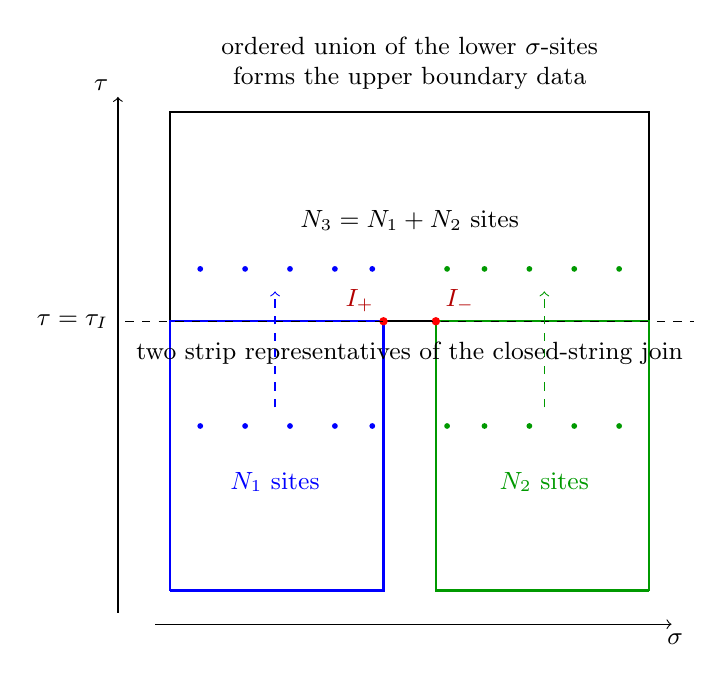
\begin{tikzpicture}[scale=0.95, every node/.style={font=\small}]
\draw[thick] (-3.2,1.6) -- (3.2,1.6) -- (3.2,4.4) -- (-3.2,4.4) -- cycle;
\draw[thick,blue] (-3.2,-2.0) -- (-3.2,1.6) -- (-0.35,1.6);
\draw[thick,blue] (-3.2,-2.0) -- (-0.35,-2.0) -- (-0.35,1.6);
\draw[thick,green!60!black] (3.2,-2.0) -- (3.2,1.6) -- (0.35,1.6);
\draw[thick,green!60!black] (3.2,-2.0) -- (0.35,-2.0) -- (0.35,1.6);
\draw[thick] (-0.35,1.6) -- (0.35,1.6);
\fill[red] (-0.35,1.6) circle (1.6pt);
\fill[red] (0.35,1.6) circle (1.6pt);
\node[red!70!black,above left] at (-0.35,1.6) {$I_+$};
\node[red!70!black,above right] at (0.35,1.6) {$I_-$};
\draw[dashed] (-3.8,1.6) -- (3.8,1.6);
\node[left] at (-3.9,1.6) {$\tau=\tau_I$};
\draw[->] (-3.9,-2.3) -- (-3.9,4.6);
\node[left] at (-3.9,4.75) {$\tau$};
\draw[->] (-3.4,-2.45) -- (3.5,-2.45);
\node[below] at (3.55,-2.45) {$\sigma$};

\foreach \x in {-2.8,-2.2,-1.6,-1.0,-0.5} {
  \fill[blue] (\x,0.2) circle (1.1pt);
  \fill[blue] (\x,2.3) circle (1.1pt);
}
\foreach \x in {0.5,1.0,1.6,2.2,2.8} {
  \fill[green!60!black] (\x,0.2) circle (1.1pt);
  \fill[green!60!black] (\x,2.3) circle (1.1pt);
}

\draw[dashed,->,blue] (-1.8,0.45) -- (-1.8,2.0);
\draw[dashed,->,green!60!black] (1.8,0.45) -- (1.8,2.0);

\node[blue] at (-1.8,-0.55) {$N_1$ sites};
\node[green!60!black] at (1.8,-0.55) {$N_2$ sites};
\node at (0,2.95) {$N_3=N_1+N_2$ sites};
\node[align=center] at (0,5.05) {ordered union of the lower $\sigma$-sites\\ forms the upper boundary data};
\node[below] at (0,1.45) {two strip representatives of the closed-string join};
\end{tikzpicture}
\caption{Cubic Mandelstam diagram in lightcone $(\tau,\sigma)$ coordinates. The two incoming strips join at the interaction time $\tau_I$ to form a single outgoing strip. Dots denote discretized $\sigma$-sites on constant-$\tau$ slices. The upper slice is the ordered concatenation of the lower left and lower right slices, so the position-space overlap is $X^{(3)}=(P_1X^{(1)}+P_2X^{(2)})$, and similarly for the kinematic fermionic overlap. The red points $I_+$ and $I_-$ are the two strip representatives of the closed-string interaction region in the unfolded picture.}
\label{fig:boundary-overlap-join}
\end{figure}

From here on, the main target is the closed string. Figure~\ref{fig:boundary-overlap-join} should therefore be read as the unfolded representation of a cut closed-string pair of pants: each actual constant-$\tau$ slice is a circle, cut open and laid out as an interval so that the $\sigma$-site concatenation is explicit. In this unfolded picture the single closed-string interaction region appears as the pair of strip endpoints $I_+$ and $I_-$ at the two ends of the cut on the outgoing strip. The holomorphic interaction-point operator $K$ is attached to the $I_+$ arc, while the antiholomorphic operator $\widetilde K$ is attached to the $I_-$ arc. For brevity I often denote the pair by a single vertex label $I$. The open-string version is the same site-space construction with only one chiral sector.

For the off-shell cubic vertex and its higher-loop sewing, however, I do \emph{not} impose level matching a priori on each internal leg. The $\sigma$-space overlap treats all Fourier modes uniformly, and the split into left- and right-movers is recovered only after Fourier transform by separating positive and negative mode numbers (with the self-conjugate middle mode when $N$ is even). Level matching is imposed only when projecting onto external on-shell closed-string states or when comparing with physical S-matrix elements; at tree level this projection is inserted explicitly on the external legs, while at loop level it is enforced in internal channels by the twist integrations.

If one works directly with GS boundary fermions, the kinematic fermionic overlap is organized by the same concatenation map:
\begin{equation}
\theta^{(3)} = P_1 \theta^{(1)} + P_2 \theta^{(2)}
\end{equation}
in $\sigma$ position space, with the same orientation conventions as for the bosons. In particular, at the interaction point itself one identifies
\begin{equation}
\theta_{I_+}^a\equiv \theta_0^{(1)a}=\theta_0^{(3)a},
\qquad
\theta_{I_-}^a\equiv \theta_0^{(2)a}=\theta_{N_1}^{(3)a},
\end{equation}
namely the two strip representatives of the local closed-string interaction region. These variables are not the average Grassmann modes on the legs. So there are not three independent endpoint spinors in the local vertex; rather, in the unfolded closed-string strip one has the pair $(\theta_{I_+},\theta_{I_-})$ together with whatever independent fermionic zero-mode or conjugate Grassmann variable remains after the full overlap constraints are solved.

\section{Position basis versus Fourier basis versus oscillators}
The cubic overlap is imposed on site values $X_n^{(r)}$ and $\theta_n^{(r)}$ in $\sigma$ position space. Comparison with conventional lightcone three-string amplitudes is obtained in two steps: first transform to nonzero discrete Fourier modes, and only then to harmonic-oscillator creation/annihilation operators.

For bosons on leg $r$ with $N_r$ lattice sites, separate center-of-mass and oscillator parts:
\begin{equation}
X_n^{(r)} = x_{\mathrm{cm}}^{(r)} + X_n^{\prime(r)},
\qquad
P_n^{(r)} = \frac{p_\perp^{(r)}}{N_r} + P_n^{\prime(r)},
\qquad
\sum_{n=0}^{N_r-1}X_n^{\prime(r)}=\sum_{n=0}^{N_r-1}P_n^{\prime(r)}=0.
\end{equation}
Then expand the zero-sum parts as
\begin{equation}
X_n^{\prime(r)} = \frac{1}{\sqrt{N_r}}\sum_{m=1}^{N_r-1} q_m^{(r)} e^{2\pi \ii mn/N_r},
\qquad
P_n^{\prime(r)} = \frac{1}{\sqrt{N_r}}\sum_{m=1}^{N_r-1} \pi_m^{(r)} e^{2\pi \ii mn/N_r}.
\end{equation}
The inverse transform is
\begin{equation}
x_{\mathrm{cm}}^{(r)} = \frac{1}{N_r}\sum_{n=0}^{N_r-1} X_n^{(r)},
\qquad
q_m^{(r)} = \frac{1}{\sqrt{N_r}}\sum_{n=0}^{N_r-1} X_n^{(r)} e^{-2\pi \ii mn/N_r},
\end{equation}
and similarly
\begin{equation}
p_\perp^{(r)} = \sum_{n=0}^{N_r-1} P_n^{(r)},
\qquad
\pi_m^{(r)} = \frac{1}{\sqrt{N_r}}\sum_{n=0}^{N_r-1} P_n^{(r)} e^{-2\pi \ii mn/N_r}.
\end{equation}
For real fields one has
\begin{equation}
q_{N_r-m}^{(r)} = \bigl(q_m^{(r)}\bigr)^*,
\qquad
\pi_{N_r-m}^{(r)} = \bigl(\pi_m^{(r)}\bigr)^*.
\end{equation}

It is convenient to package the nonzero Fourier modes into the rectangular DFT matrix
\begin{equation}
(\widehat F_r)_{mn} = \frac{1}{\sqrt{N_r}} e^{-2\pi \ii mn/N_r},
\qquad
m=1,\dots,N_r-1,\quad n=0,\dots,N_r-1,
\end{equation}
so that
\begin{equation}
X^{(r)} = x_{\mathrm{cm}}^{(r)}{\bf 1}_{N_r} + \widehat F_r^\dagger q^{(r)},
\qquad
P^{(r)} = \frac{p_\perp^{(r)}}{N_r}{\bf 1}_{N_r} + \widehat F_r^\dagger \pi^{(r)}.
\end{equation}

The full-boundary overlap implies the weighted center-of-mass relation
\begin{equation}
N_3 x_{\mathrm{cm}}^{(3)} = N_1 x_{\mathrm{cm}}^{(1)} + N_2 x_{\mathrm{cm}}^{(2)},
\end{equation}
and the oscillator sector obeys an \emph{affine} rather than homogeneous relation,
\begin{equation}
q^{(3)} = U_1 q^{(1)} + U_2 q^{(2)} + \xi\,y,
\qquad
y\equiv x_{\mathrm{cm}}^{(1)}-x_{\mathrm{cm}}^{(2)},
\end{equation}
with
\begin{equation}
U_r \equiv \widehat F_3 P_r \widehat F_r^\dagger,
\qquad
\xi \equiv \widehat F_3 P_1 {\bf 1}_{N_1}
= -\widehat F_3 P_2 {\bf 1}_{N_2}.
\end{equation}
So the nonzero Fourier modes are determined by the site-basis overlap together with the relative center-of-mass displacement $y$. This is the discrete counterpart of the fact that continuum three-string vertices contain both quadratic Neumann coefficients and linear zero-mode couplings.

The matrix elements are completely explicit:
\begin{equation}
(U_1)_{m\ell}
=
\frac{1}{\sqrt{N_3 N_1}}
\sum_{n=0}^{N_1-1}
e^{-2\pi \ii mn/N_3} e^{2\pi \ii \ell n/N_1},
\end{equation}
\begin{equation}
(U_2)_{m\ell}
=
\frac{1}{\sqrt{N_3 N_2}}
\sum_{n=0}^{N_2-1}
e^{-2\pi \ii m(n+N_1)/N_3} e^{2\pi \ii \ell n/N_2}.
\end{equation}
The second matrix carries the expected phase offset coming from the fact that the second string occupies the interval $\sigma\in[\alpha_1,\alpha_3]$ on the outgoing leg. The center-of-mass mixing vector is equally explicit:
\begin{equation}
\xi_m
=
\frac{1}{\sqrt{N_3}}
\sum_{n=0}^{N_1-1}
e^{-2\pi \ii mn/N_3}
=
\frac{1-e^{-2\pi \ii m N_1/N_3}}{\sqrt{N_3}\,\bigl(1-e^{-2\pi \ii m/N_3}\bigr)},
\qquad
m=1,\dots,N_3-1.
\end{equation}

To compare directly with oscillator formulas, define for each nonzero mode
\begin{equation}
a_m^{(r)}
=
\sqrt{\frac{\mu_r\omega_m^{(r)}}{2}}\,q_m^{(r)}
\,+\,
\frac{\ii}{\sqrt{2\mu_r\omega_m^{(r)}}}\,\pi_m^{(r)},
\qquad
\mu_r=\frac{a_r}{2\pi\al}.
\end{equation}
Equivalently, the exact site-to-oscillator map is
\begin{equation}
\begin{aligned}
a_m^{(r)}
=
\frac{1}{\sqrt{N_r}}
\sum_{n=0}^{N_r-1}
\left[
\sqrt{\frac{\mu_r\omega_m^{(r)}}{2}}\,X_n^{\prime(r)}
+\frac{\ii}{\sqrt{2\mu_r\omega_m^{(r)}}}\,P_n^{\prime(r)}
\right]
e^{-2\pi \ii mn/N_r}.
\end{aligned}
\end{equation}
The inverse formulas are
\begin{equation}
\begin{aligned}
X_n^{\prime(r)}
&=
\frac{1}{\sqrt{N_r}}
\sum_{m=1}^{N_r-1}
\frac{a_m^{(r)}+a_{N_r-m}^{(r)\dagger}}{\sqrt{2\mu_r\omega_m^{(r)}}}
e^{2\pi \ii mn/N_r},\\
P_n^{\prime(r)}
&=
\frac{-\ii}{\sqrt{N_r}}
\sum_{m=1}^{N_r-1}
\sqrt{\frac{\mu_r\omega_m^{(r)}}{2}}\,
\bigl(a_m^{(r)}-a_{N_r-m}^{(r)\dagger}\bigr)
e^{2\pi \ii mn/N_r}.
\end{aligned}
\end{equation}
The DFT convention implies the canonical commutator
\begin{equation}
\bigl[q_m^{(r)},\pi_n^{(s)}\bigr]
=
\mathrm{i}\,\delta^{rs}\delta_{m,N_r-n},
\end{equation}
with all other commutators vanishing on the nonzero-mode sector. Consequently,
\begin{equation}
\bigl[a_m^{(r)},a_n^{(s)\dagger}\bigr]
=
\delta^{rs}\delta_{mn},
\qquad
\text{equivalently}
\qquad
\bigl[a_m^{(r)},a_{N_r-n}^{(s)}\bigr]
=
\delta^{rs}\delta_{mn}
\end{equation}
on physical states, because the Hermitian adjoint is represented in the complexified basis by the anti-linear involution $m\mapsto N_r-m$.
In these formulas I keep the full complexified nonzero Fourier basis $m=1,\dots,N_r-1$. Reality of the original site field is imposed by the anti-linear involution
\begin{equation}
q_{N_r-m}^{(r)}=\bigl(q_m^{(r)}\bigr)^*,
\qquad
\pi_{N_r-m}^{(r)}=\bigl(\pi_m^{(r)}\bigr)^*,
\qquad
a_{N_r-m}^{(r)}=\bigl(a_m^{(r)}\bigr)^\dagger,
\end{equation}
on physical states. Equivalently, one may restrict to an independent half-spectrum. In the complexified basis, the overlap and squeezed-state formulas are written on all nonzero modes, with the understanding that the resulting squeeze matrix respects this involution.

For fermions one uses the same DFT matrices. Writing
\begin{equation}
\theta_n^{(r)}=\theta_{\mathrm{av}}^{(r)}+\frac{1}{\sqrt{N_r}}\sum_{m=1}^{N_r-1}\vartheta_m^{(r)}e^{2\pi \ii mn/N_r},
\end{equation}
the average Grassmann mode obeys
\begin{equation}
N_3\theta_{\mathrm{av}}^{(3)}=N_1\theta_{\mathrm{av}}^{(1)}+N_2\theta_{\mathrm{av}}^{(2)},
\end{equation}
and if one keeps the relative average Grassmann mode
\begin{equation}
\upsilon\equiv \theta_{\mathrm{av}}^{(1)}-\theta_{\mathrm{av}}^{(2)},
\end{equation}
explicit, then the nonzero Fourier modes obey the same affine overlap pattern as the bosons,
\begin{equation}
\vartheta^{(3)} = U_1 \vartheta^{(1)} + U_2 \vartheta^{(2)} + \xi\,\upsilon.
\end{equation}
In a coherent-state oscillator basis this affine Grassmann term becomes the corresponding linear source in the displaced fermionic squeezed state. So both the bosonic and fermionic cubic vertices are defined most naturally in $\sigma$ position space, while the familiar oscillator-basis data are obtained by the explicit DFT maps above.

Figure~\ref{fig:basis-map} summarizes the bookkeeping: the discretized calculation is done in site variables, while comparison with conventional string-amplitude formulas is made after the explicit DFT and oscillator transforms.

\begin{figure}[t]
\centering
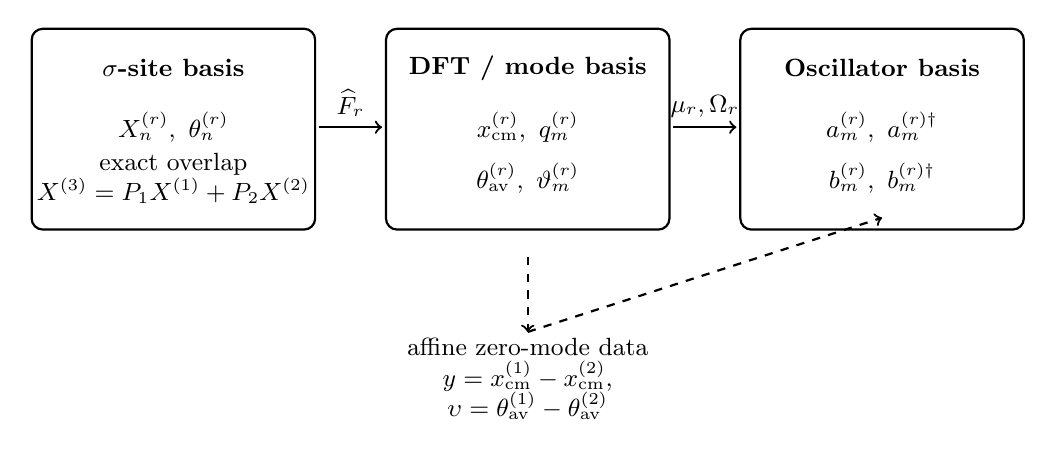
\begin{tikzpicture}[scale=1.0, every node/.style={font=\small}]
\draw[thick,rounded corners] (-5.3,-1.1) rectangle (-1.7,1.45);
\draw[thick,rounded corners] (-0.8,-1.1) rectangle (2.8,1.45);
\draw[thick,rounded corners] (3.7,-1.1) rectangle (7.3,1.45);

\node[align=center] at (-3.5,0.95) {\textbf{$\sigma$-site basis}};
\node[align=center] at (-3.5,0.2) {$X_n^{(r)},\ \theta_n^{(r)}$};
\node[align=center] at (-3.5,-0.45) {exact overlap\\ $X^{(3)}=P_1X^{(1)}+P_2X^{(2)}$};

\node[align=center] at (1.0,0.95) {\textbf{DFT / mode basis}};
\node[align=center] at (1.0,0.2) {$x_{\mathrm{cm}}^{(r)},\ q_m^{(r)}$};
\node[align=center] at (1.0,-0.45) {$\theta_{\mathrm{av}}^{(r)},\ \vartheta_m^{(r)}$};

\node[align=center] at (5.5,0.95) {\textbf{Oscillator basis}};
\node[align=center] at (5.5,0.2) {$a_m^{(r)},\ a_m^{(r)\dagger}$};
\node[align=center] at (5.5,-0.45) {$b_m^{(r)},\ b_m^{(r)\dagger}$};

\draw[->,thick] (-1.65,0.2) -- node[above] {$\widehat F_r$} (-0.85,0.2);
\draw[->,thick] (2.85,0.2) -- node[above] {$\mu_r,\Omega_r$} (3.65,0.2);

\draw[->,thick,dashed] (1.0,-1.45) -- (1.0,-2.4);
\node[align=center] at (1.0,-3.0) {affine zero-mode data\\ $y=x_{\mathrm{cm}}^{(1)}-x_{\mathrm{cm}}^{(2)}$,\\ $\upsilon=\theta_{\mathrm{av}}^{(1)}-\theta_{\mathrm{av}}^{(2)}$};
\draw[->,thick,dashed] (1.0,-2.4) -- (5.5,-0.95);
\end{tikzpicture}
\caption{Three equivalent descriptions of the same cubic data. The numerical sewing problem is posed in $\sigma$ position space, then transformed to nonzero Fourier modes, and finally to creation/annihilation variables for direct comparison with the usual lightcone vertex. The affine zero-mode data survive this chain as source terms rather than as part of the homogeneous oscillator overlap.}
\label{fig:basis-map}
\end{figure}

\section{Bosonic cubic vertex in oscillator basis}
The exact position-space overlap state is
\begin{equation}
\langle X^{(1)},X^{(2)},X^{(3)}|V_3^{(B)}\rangle
=
\delta\!\bigl(X^{(3)}-P_1X^{(1)}-P_2X^{(2)}\bigr).
\end{equation}
After separating center-of-mass and oscillator variables, this becomes
\begin{equation}
\delta\!\left(
x_{\mathrm{cm}}^{(3)}-\frac{N_1x_{\mathrm{cm}}^{(1)}+N_2x_{\mathrm{cm}}^{(2)}}{N_3}
\right)
\,
\delta\!\left(q^{(3)}-U_1q^{(1)}-U_2q^{(2)}-\xi y\right),
\end{equation}
with $y=x_{\mathrm{cm}}^{(1)}-x_{\mathrm{cm}}^{(2)}$. If one Fourier transforms the center-of-mass variables to momentum space, the first delta becomes the usual transverse momentum conservation factor
\begin{equation}
\delta^{(\perpD)}\!\left(p_\perp^{(1)}+p_\perp^{(2)}-p_\perp^{(3)}\right),
\end{equation}
while the second delta produces the familiar zero-mode-dependent linear terms in the oscillator vertex. This is the discrete version of the standard continuum three-string structure.

Canonical invariance of the one-form
\begin{equation}
\sum_{r=1}^3 \epsilon_r\, P^{(r)} \cdot \delta X^{(r)},
\qquad
(\epsilon_1,\epsilon_2,\epsilon_3)=(+1,+1,-1),
\end{equation}
restricted to the oscillator sector then gives the conjugate momentum overlap
\begin{equation}
\pi^{(1)} = U_1^\dagger \pi^{(3)},
\qquad
\pi^{(2)} = U_2^\dagger \pi^{(3)}.
\end{equation}
Here the variation is taken at fixed zero-mode data, so $\delta y=0$ in the oscillator derivation. The center-of-mass momentum conservation is handled separately by Fourier transforming the weighted center-of-mass overlap, which yields the factor $\delta^{(\perpD)}(p_\perp^{(1)}+p_\perp^{(2)}-p_\perp^{(3)})$ already displayed above.

Define oscillator annihilation operators on each leg by
\begin{equation}
a^{(r)} =
\frac{1}{\sqrt2}\left(
(\mu_r\Omega_r)^{1/2} q^{(r)}
\,+\,
\ii\,(\mu_r\Omega_r)^{-1/2}\pi^{(r)}
\right),
\qquad
\Omega_r = \mathrm{diag}\!\bigl(\omega_m^{(r)}\bigr)_{m=1}^{N_r-1},
\end{equation}
and collect them into one column vector
\begin{equation}
A =
\begin{pmatrix}
a^{(1)}\\
a^{(2)}\\
a^{(3)}
\end{pmatrix},
\qquad
\mu=\mathrm{diag}(\mu_1 I,\mu_2 I,\mu_3 I),
\qquad
\Omega = \mathrm{diag}(\Omega_1,\Omega_2,\Omega_3).
\end{equation}
Introduce the coordinate and momentum overlap matrices
\begin{equation}
C_Q=
\begin{pmatrix}
U_1 & U_2 & -I
\end{pmatrix},
\qquad
C_P=
\begin{pmatrix}
I & 0 & -U_1^\dagger \\
0 & I & -U_2^\dagger
\end{pmatrix}.
\end{equation}
The homogeneous part of the overlap conditions is equivalent to
\begin{equation}
(\mathbb M A + \mathbb N A^\dagger)\,|V_3^{(B)}\rangle = 0,
\end{equation}
with
\begin{equation}
\mathbb M =
\begin{pmatrix}
 C_Q (\mu\Omega)^{-1/2}\\
 -\ii C_P (\mu\Omega)^{1/2}
\end{pmatrix},
\qquad
\mathbb N =
\begin{pmatrix}
 C_Q (\mu\Omega)^{-1/2}\\
 \ii C_P (\mu\Omega)^{1/2}
\end{pmatrix}.
\end{equation}
Because the position-space sewing is affine on the oscillator variables, the full constraint at fixed relative center-of-mass coordinate $y$ is actually
\begin{equation}
(\mathbb M A + \mathbb N A^\dagger + J_0(y))\,|V_3^{(B)}\rangle = 0,
\end{equation}
where in the convention used here, with the center-of-mass coordinate Fourier transformed to transverse momentum and only the relative displacement $y=x_{\mathrm{cm}}^{(1)}-x_{\mathrm{cm}}^{(2)}$ left explicit,
\begin{equation}
J_0(y)=
\begin{pmatrix}
\sqrt2\,\xi\,y\\
0
\end{pmatrix}.
\end{equation}
The upper block comes from the affine coordinate overlap $C_Qq=-\xi y$, while the lower block vanishes because the oscillator momentum overlap is homogeneous. In a different zero-mode basis the source vector is obtained from this one by a linear change of variables. The constraint count is
\begin{equation}
N_{\mathrm{rows}}(C_Q)+N_{\mathrm{rows}}(C_P)
=(N_3-1)+(N_1-1+N_2-1)=2N_3-3,
\end{equation}
which exactly matches the number of oscillator variables on the three legs. Since each $(\mu_r\Omega_r)^{\pm1/2}$ is invertible on the nonzero-mode sector, nondegeneracy of $\mathbb M$ reduces to linear independence of these exact overlap constraints. This is a finite-dimensional statement that can and should be checked numerically at each lattice resolution $N$. Assuming $\mathbb M$ is nondegenerate on the oscillator subspace, the exact solution is a displaced squeezed state
\begin{equation}
|V_3^{(B)}\rangle =
{\cal C}_3^{(B)}
\delta^{(\perpD)}(p_\perp^{(1)}+p_\perp^{(2)}-p_\perp^{(3)})
\exp\!\left[
 -\frac12 A^{\dagger T}\,S^{(B)}\,A^\dagger
 -A^{\dagger T}\Lambda^{(B)}(y)
 -\frac12\Phi^{(B)}(y)
\right]|0\rangle,
\end{equation}
with
\begin{equation}
S^{(B)} = -\mathbb M^{-1}\mathbb N,
\qquad
\Lambda^{(B)} = -\mathbb M^{-1}J_0,
\end{equation}
while $\Phi^{(B)}(y)$ is the scalar normal-ordering completion. The overall constant ${\cal C}_3^{(B)}$ is likewise not fixed by the annihilation equations alone: at finite $N$ it is a lattice-resolution-dependent analogue of the Mandelstam local normalization and must be fixed by the same Poincare-algebra check that fixes the continuum cubic vertex normalization. Equivalently, one may define $\Phi^{(B)}(y)$ by
\begin{equation}
e^{-\Phi^{(B)}(y)/2}
\equiv
\frac{\langle 0|V_3^{(B)}(y)\rangle}
{{\cal C}_3^{(B)}\,
\delta^{(\perpD)}(p_\perp^{(1)}+p_\perp^{(2)}-p_\perp^{(3)})},
\end{equation}
so $\Phi^{(B)}(y)$ is a quadratic form in the relative center-of-mass displacement $y$ determined uniquely once the exact overlap state is normalized. The matrix $S^{(B)}$ is the full oscillator squeeze matrix of the vertex. If $\mathcal R=\mathrm{diag}(\mathcal R_1,\mathcal R_2,\mathcal R_3)$ with $(\mathcal R_r)_{mn}=\delta_{m,N_r-n}$, reality requires
\begin{equation}
S^{(B)}=\mathcal R\,S^{(B)*}\,\mathcal R,
\qquad
\Lambda^{(B)}=\mathcal R\,\Lambda^{(B)*}.
\end{equation}
The reduced discrete Neumann coefficients used for continuum comparison are extracted from $S^{(B)}$ only after the affine zero-mode pieces have been separated.

\section{Bosonic Lorentz check}
In lightcone gauge, the cubic Hamiltonian and Lorentz generators are expanded as
\begin{equation}
P^- = P^-_2 + g P^-_3 + O(g^2),
\qquad
J^{-I} = J^{-I}_2 + g J^{-I}_3 + O(g^2).
\end{equation}
At order $g$, Lorentz invariance requires
\begin{equation}
[J^{-I}_2,P^-_3] + [J^{-I}_3,P^-_2] = 0,
\qquad
[J^{-I}_2,J^{-J}_3] + [J^{-I}_3,J^{-J}_2] = 0.
\end{equation}

The kinematical generators are straightforward:
\begin{itemize}
\item $P^+$ is conserved because $N_3=N_1+N_2$, equivalently $\alpha_3=\alpha_1+\alpha_2$ in the positive-circumference notation introduced in Section~4.
\item $P^I$ is conserved because the zero-mode overlap gives $\delta^{(\perpD)}(p_\perp^{(1)}+p_\perp^{(2)}-p_\perp^{(3)})$.
\item $J^{IJ}$ is automatic because the overlap state is an SO$(D-2)$ scalar in the transverse indices.
\item $J^{+I}$ follows from the weighted center-of-mass relation together with $P^+$ conservation.
\end{itemize}
Indeed, since $p_r^+=\alpha_r/(2\alpha')$ in that same positive-circumference notation, the weighted identity $\alpha_3 x_{\mathrm{cm}}^{(3)}=\alpha_1 x_{\mathrm{cm}}^{(1)}+\alpha_2 x_{\mathrm{cm}}^{(2)}$ is precisely the condition needed for the center-of-mass part of $J^{+I}$ to sew consistently across the cubic vertex.

The nontrivial test is the dynamical generator. For the closed bosonic string,
\begin{equation}
J^{-I}_2
=
x^- p^I
-\frac12 \{x^I,P^-_2\}
+\frac{\ii}{p^+}\sum_{n\ge 1}\frac{1}{n}
\left(
\alpha_{-n}^I L_n - L_{-n}\alpha_n^I
+\tilde\alpha_{-n}^I \tilde L_n - \tilde L_{-n}\tilde\alpha_n^I
\right),
\end{equation}
with the usual chiral normal-ordering constants $a_L=a_R=1$. Acting on the overlap state, the bulk pieces cancel because the $\sigma$-space sewing is exact. The only possible obstruction is a join-local normal-ordering anomaly. In the continuum this anomaly cancels precisely for
\begin{equation}
D=26,
\qquad
a_L=a_R=1
\quad
(\text{equivalently total intercept }2),
\end{equation}
together with the standard Mandelstam normalization of the cubic vertex. The discrete check is therefore:
\begin{enumerate}
\item build $|V_3^{(B)}\rangle$ from the exact $\sigma$-space overlap,
\item evaluate the lattice version of $[J^{-I}_2,P^-_3] + [J^{-I}_3,P^-_2]$,
\item isolate the residual join-local term,
\item verify that its continuum limit reproduces the usual critical-dimension constraint.
\end{enumerate}
So the bosonic cubic vertex is not just the overlap state: it is the overlap state with the normalization and oscillator ordering fixed so that the lightcone Poincare algebra closes.

\section{Fermionic kinematic overlap}
The fermionic part should be treated in complete parallel with the bosons. Let $\theta^{(r)}$ denote the GS worldsheet fermions on leg $r$ in $\sigma$ position space. The full-boundary overlap gives
\begin{equation}
\theta^{(3)} = P_1 \theta^{(1)} + P_2 \theta^{(2)},
\end{equation}
including the two unfolded-strip representatives $\theta_{I_+}$ and $\theta_{I_-}$ discussed above. In a coherent-state basis, the kinematic fermionic vertex is therefore the Grassmann delta functional
\begin{equation}
\langle \bar\theta^{(1)},\bar\theta^{(2)},\bar\theta^{(3)} | V^{(F)}_{\mathrm{kin}} \rangle
\propto
\delta\!\left(\bar\theta^{(3)}-\bar\theta^{(1)}P_1^T-\bar\theta^{(2)}P_2^T\right).
\end{equation}

Removing the average mode and transforming to nonzero Fourier modes gives
\begin{equation}
\vartheta^{(3)} = U_1 \vartheta^{(1)} + U_2 \vartheta^{(2)} + \xi\,\upsilon,
\qquad
\upsilon\equiv \theta_{\mathrm{av}}^{(1)}-\theta_{\mathrm{av}}^{(2)},
\end{equation}
with the same overlap matrices $U_r=\widehat F_3P_r\widehat F_r^\dagger$ and affine vector $\xi$ as in the bosonic sector. In a coherent-state oscillator basis this becomes a displaced fermionic squeezed state. After shifting away the affine zero-mode source, one may write the homogeneous part in terms of oscillator variables $b^{(r)}$ as
\begin{equation}
b^{(3)} = U_1 b^{(1)} + U_2 b^{(2)},
\end{equation}
or, in a canonical first-order phase-space basis for the real nonzero fermionic modes,
\begin{equation}
\vartheta_m^{(r)}=\frac{b_m^{(r)}+b_{N_r-m}^{(r)\dagger}}{\sqrt2},
\qquad
\pi_{\vartheta,m}^{(r)}=\frac{b_m^{(r)}-b_{N_r-m}^{(r)\dagger}}{\mathrm{i}\sqrt2},
\end{equation}
with anticommutator
\begin{equation}
\bigl\{\vartheta_m^{(r)},\pi_{\vartheta,n}^{(s)}\bigr\}
=
\mathrm{i}\,\delta^{rs}\delta_{m,N_r-n}.
\end{equation}
Then the fermionic overlap matrices are explicitly
\begin{equation}
C_{\Theta}=
\begin{pmatrix}
U_1 & U_2 & -I
\end{pmatrix},
\qquad
C_{\Pi_{\Theta}}=
\begin{pmatrix}
I & 0 & -U_1^\dagger\\
0 & I & -U_2^\dagger
\end{pmatrix},
\end{equation}
and therefore
\begin{equation}
\mathbb M_F=
\begin{pmatrix}
C_{\Theta}\\
-\mathrm{i}C_{\Pi_{\Theta}}
\end{pmatrix},
\qquad
\mathbb N_F=
\begin{pmatrix}
C_{\Theta}\\
\mathrm{i}C_{\Pi_{\Theta}}
\end{pmatrix}.
\end{equation}
This is the fermionic analogue of the bosonic overlap system, without the frequency factors $(\mu\Omega)^{\pm1/2}$ because the GS fermions are first order rather than second order in worldsheet time.
Equivalently, the kinematic overlap state solves linear constraints of the form
\begin{equation}
(\mathbb M_F B + \mathbb N_F B^\dagger)\,|V^{(F)}_{\mathrm{kin}}\rangle = 0,
\end{equation}
for the collective fermionic oscillator vector
\begin{equation}
B =
\begin{pmatrix}
b^{(1)}\\
b^{(2)}\\
b^{(3)}
\end{pmatrix},
\end{equation}
and hence
\begin{equation}
|V^{(F)}_{\mathrm{kin}}\rangle
=
{\cal C}_3^{(F)}
\exp\!\left[
\frac12 B^{\dagger T}S^{(F)} B^\dagger
\right]|0\rangle,
\qquad
S^{(F)} = -\mathbb M_F^{-1}\mathbb N_F.
\end{equation}
Thus the superstring cubic vertex factorizes into a kinematic overlap state
\begin{equation}
|V_{\mathrm{kin}}\rangle = |V_3^{(B)}\rangle \otimes |V^{(F)}_{\mathrm{kin}}\rangle
\end{equation}
times the local interaction-point prefactor. The omitted affine fermionic source is carried entirely by the surviving zero-mode combination $\upsilon$, which later becomes part of the local GS variable $\Lambda_{\mathrm{lat}}$.

For numerical work one must also fix the Grassmann ordering convention once and for all. A convenient choice is to order variables by leg, then by site, then by SO$(8)$ index:
\begin{equation}
\Theta=
\bigl(
\theta^{(1)}_{0,1},\dots,\theta^{(1)}_{N_1-1,8};
\theta^{(2)}_{0,1},\dots,\theta^{(2)}_{N_2-1,8};
\theta^{(3)}_{0,1},\dots,\theta^{(3)}_{N_3-1,8}
\bigr).
\end{equation}
The Berezin measure is taken in the matching order. Once this convention is fixed, the overall sign of every fermionic determinant/Pfaffian is fixed consistently across all diagrams.

\section{Superstring cubic vertex and GS prefactor}
In the superstring, the full cubic vertex is not an arbitrary polynomial ansatz. One should first construct the kinematic overlap state $|V_{\mathrm{kin}}\rangle$ implementing the exact bosonic and fermionic boundary concatenation, and only then multiply by the local Green--Schwarz prefactor:
\begin{equation}
|V_{\mathrm{GS}}\rangle
=
{\cal P}_I\,\widetilde{\cal P}_I\,|V_{\mathrm{kin}}\rangle.
\end{equation}
The prefactor is fixed, up to overall normalization and possible finite-$a$ counterterms, by the requirement that the dynamical supercharges act correctly on the vertex:
\begin{equation}
\left(\sum_{r=1}^3 Q_r^-\right)|V_{\mathrm{GS}}\rangle=0,
\qquad
\left(\sum_{r=1}^3 \widetilde Q_r^-\right)|V_{\mathrm{GS}}\rangle=0.
\end{equation}
Thus low-point amplitudes are checks of the construction, not the primary definition of the vertex.

In the unfolded closed-string strip, define the two local representatives
\begin{equation}
X_{I_+}\equiv X_0^{(1)}=X_0^{(3)},
\qquad
X_{I_-}\equiv X_0^{(2)}=X_{N_1}^{(3)},
\end{equation}
and likewise
\begin{equation}
\theta_{I_+}\equiv \theta_0^{(1)}=\theta_0^{(3)},
\qquad
\theta_{I_-}\equiv \theta_0^{(2)}=\theta_{N_1}^{(3)}.
\end{equation}
The raw local lattice data are then the one-sided differences on the two arcs,
\begin{equation}
\nabla_+ X^{(1)}_{I_+} \equiv X^{(1)}_1-X_{I_+},
\qquad
\nabla_+ X^{(3)}_{I_+} \equiv X^{(3)}_1-X_{I_+},
\end{equation}
\begin{equation}
\nabla_- X^{(2)}_{I_-} \equiv X_{I_-}-X^{(2)}_{N_2-1},
\qquad
\nabla_- X^{(3)}_{I_-} \equiv X_{I_-}-X^{(3)}_{N_3-1},
\end{equation}
and similarly
\begin{equation}
\nabla_+ \theta^{(1)}_{I_+} \equiv \theta^{(1)}_1-\theta_{I_+},
\qquad
\nabla_+ \theta^{(3)}_{I_+} \equiv \theta^{(3)}_1-\theta_{I_+},
\end{equation}
\begin{equation}
\nabla_- \theta^{(2)}_{I_-} \equiv \theta_{I_-}-\theta^{(2)}_{N_2-1},
\qquad
\nabla_- \theta^{(3)}_{I_-} \equiv \theta_{I_-}-\theta^{(3)}_{N_3-1}.
\end{equation}
These are \emph{not} yet the continuum interaction-point operators $K^I$ and $\widetilde K^I$; they are only the finite lattice differences from which those singular operators must be reconstructed.

Figure~\ref{fig:interaction-arcs} isolates the local geometry relevant for the interaction-point prefactor. The two operators probe different arcs of the unfolded closed-string join.

\begin{figure}[t]
\centering
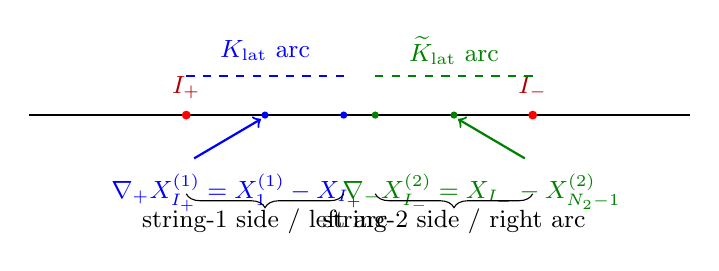
\begin{tikzpicture}[scale=1.0, every node/.style={font=\small}]
\draw[thick] (-4.2,0) -- (4.2,0);
\fill[red] (-2.2,0) circle (1.6pt);
\fill[red] (2.2,0) circle (1.6pt);
\node[red!70!black,above] at (-2.2,0.08) {$I_+$};
\node[red!70!black,above] at (2.2,0.08) {$I_-$};

\fill[blue] (-1.2,0) circle (1.3pt);
\fill[blue] (-0.2,0) circle (1.3pt);
\fill[green!50!black] (1.2,0) circle (1.3pt);
\fill[green!50!black] (0.2,0) circle (1.3pt);

\draw[->,thick,blue] (-2.1,-0.55) -- (-1.25,-0.05);
\node[blue,below] at (-1.55,-0.62) {$\nabla_+X^{(1)}_{I_+}=X_1^{(1)}-X_{I_+}$};
\draw[->,thick,green!50!black] (2.1,-0.55) -- (1.25,-0.05);
\node[green!50!black,below] at (1.55,-0.62) {$\nabla_-X^{(2)}_{I_-}=X_{I_-}-X_{N_2-1}^{(2)}$};

\draw[thick,dashed,blue] (-2.2,0.5) -- (-0.2,0.5);
\draw[thick,dashed,green!50!black] (2.2,0.5) -- (0.2,0.5);
\node[blue] at (-1.2,0.82) {$K_{\mathrm{lat}}$ arc};
\node[green!50!black] at (1.2,0.82) {$\widetilde K_{\mathrm{lat}}$ arc};

\draw[decorate,decoration={brace,mirror,amplitude=5pt}] (-2.2,-1.0) -- (-0.2,-1.0);
\draw[decorate,decoration={brace,mirror,amplitude=5pt}] (0.2,-1.0) -- (2.2,-1.0);
\node at (-1.2,-1.35) {string-1 side / left arc};
\node at (1.2,-1.35) {string-2 side / right arc};
\end{tikzpicture}
\caption{Local interaction-region geometry in the unfolded closed-string strip. The holomorphic operator $K_{\mathrm{lat}}$ probes the $I_+$ arc by a one-sided difference toward string 1, while the antiholomorphic operator $\widetilde K_{\mathrm{lat}}$ probes the $I_-$ arc by a one-sided difference toward string 2. Genuine improved stencils must stay on the same arc and involve additional nearby lattice sites.}
\label{fig:interaction-arcs}
\end{figure}

Near a continuum interaction point $z_I$, the Mandelstam map has the local form
\begin{equation}
\rho(z)=\rho_I+\frac12 \rho''(z_I)(z-z_I)^2+O\!\bigl((z-z_I)^3\bigr).
\end{equation}
Therefore $K^I$ and $\widetilde K^I$ extract the square-root singular parts of $\partial X^I$ and $\bar\partial X^I$ in the local coordinate and are not ordinary derivatives. On the lattice this means that the correct operators must be renormalized linear combinations of the raw one-sided differences with an explicit $a^{-1/2}$ scaling:
\begin{equation}
\begin{aligned}
K^I_{\mathrm{lat}}
&=
a^{-1/2}c_K\,\bigl(\nabla_+ X_{I_+}^{(1)}\bigr)^I
=
a^{-1/2}c_K\,\bigl(\nabla_+ X_{I_+}^{(3)}\bigr)^I
+O(a^{1/2}),\\
\widetilde K^I_{\mathrm{lat}}
&=
a^{-1/2}\widetilde c_K\,\bigl(\nabla_- X_{I_-}^{(2)}\bigr)^I
=
a^{-1/2}\widetilde c_K\,\bigl(\nabla_- X_{I_-}^{(3)}\bigr)^I
+O(a^{1/2}).
\end{aligned}
\end{equation}
Here the equalities use the position-space overlap itself: $\nabla_+X_{I_+}^{(3)}=\nabla_+X_{I_+}^{(1)}$ because the first site on string $3$ is the first site on string $1$, while $\nabla_-X_{I_-}^{(3)}=\nabla_-X_{I_-}^{(2)}$ because the last site on string $3$ is the last site on string $2$. Thus $K$ probes the $I_+$ arc of the join and $\widetilde K$ probes the $I_-$ arc. More general improved lattice definitions are possible,
\begin{equation}
K^I_{\mathrm{lat,imp}}
=
a^{-1/2}c_K^{(2)}\,\bigl(D^{(2)}_{I_+}X^{(1)}\bigr)^I,
\qquad
\widetilde K^I_{\mathrm{lat,imp}}
=
a^{-1/2}\widetilde c_K^{(2)}\,\bigl(\widetilde D^{(2)}_{I_-}X^{(2)}\bigr)^I,
\end{equation}
where a genuine improvement must involve extra sites on the same arc, for example the one-sided second-order stencils
\begin{equation}
D^{(2)}_{I_+}X^{(1)} \equiv \frac{-3X_{I_+}+4X_1^{(1)}-X_2^{(1)}}{2},
\qquad
\widetilde D^{(2)}_{I_-}X^{(2)} \equiv \frac{3X_{I_-}-4X_{N_2-1}^{(2)}+X_{N_2-2}^{(2)}}{2}.
\end{equation}
Because $\nabla_+X_{I_+}^{(1)}=\nabla_+X_{I_+}^{(3)}$ and $\nabla_-X_{I_-}^{(2)}=\nabla_-X_{I_-}^{(3)}$ exactly by overlap, linear combinations of those equal nearest-neighbor differences do not produce any actual improvement. Additional moment conditions on the multi-site stencil may be imposed to cancel the first $O(a^{1/2})$ corrections and improve finite-$a$ convergence. The constants $c_K$, $\widetilde c_K$, $c_K^{(2)}$, $\widetilde c_K^{(2)}$ and any higher-stencil coefficients are fixed by the local quadratic part of the Mandelstam map and by the dynamical supercharge equations; they are not free fit parameters.

The continuum lightcone GS vertex is already known. In modern notation one writes the cubic Hamiltonian schematically as
\begin{equation}
|H_3\rangle
=
{\cal C}_3^{(S)}
K^I \widetilde K^J v_{IJ}(\Lambda)
|V_{\mathrm{kin}}\rangle,
\end{equation}
where:
\begin{itemize}
\item $\Lambda^a$, $a=1,\dots,8$, are the eight independent SO$(8)$ fermionic zero-mode combinations surviving the kinematic overlap,
\item $v_{IJ}(\Lambda)$ is the known octic SO$(8)$-covariant polynomial in $\Lambda$,
\item $K^I$ and $\widetilde K^J$ are the bosonic interaction-point operators, i.e. the singular parts of $\partial X^I$ and $\bar\partial X^J$ at the join.
\end{itemize}
In the schematic formulas below, $\Lambda^a$ is taken to transform as a chiral SO$(8)$ spinor, say $\mathbf{8}_s$. For type IIA/IIB the usual relative chirality assignments between left and right sectors must be restored, but that distinction is not needed for the lattice kinematics being developed here.
The polynomial may be written schematically as
\begin{equation}
v_{IJ}(\Lambda)
=
A^{(0)}_{IJ}
+A^{(2)}_{IJ,ab}\Lambda^a\Lambda^b
+A^{(4)}_{IJ,abcd}\Lambda^a\Lambda^b\Lambda^c\Lambda^d
+A^{(6)}_{IJ,a_1\cdots a_6}\Lambda^{a_1}\cdots\Lambda^{a_6}
+A^{(8)}_{IJ}\epsilon_{a_1\cdots a_8}\Lambda^{a_1}\cdots\Lambda^{a_8},
\end{equation}
with the coefficients built from SO$(8)$ gamma matrices and the Levi-Civita tensor. Explicit formulas are available in the continuum lightcone literature \cite{SpradlinVolovich2002,PankiewiczStefanski2002}. The matrix-string interpretation of the same structure is discussed in \cite{DijkgraafMotl2003,Kishimoto2006}.

After imposing the kinematic overlap, the local fermionic data in the unfolded strip consist of the pair of strip representatives $\theta_{I_+}^a$, $\theta_{I_-}^a$ together with the surviving independent Grassmann zero-mode combination $\Lambda_{\mathrm{lat}}^a$ (or the canonically equivalent conjugate variable, depending on conventions). The lattice prefactor is therefore local to the interaction region, but not a polynomial in three independent endpoint spinors:
\begin{equation}
v_{IJ}^{\mathrm{lat}}(\Lambda_{\mathrm{lat}})
=
A^{(0)}_{IJ}
+A^{(2)}_{IJ,ab}\Lambda_{\mathrm{lat}}^a\Lambda_{\mathrm{lat}}^b
+A^{(4)}_{IJ,abcd}\Lambda_{\mathrm{lat}}^a\Lambda_{\mathrm{lat}}^b\Lambda_{\mathrm{lat}}^c\Lambda_{\mathrm{lat}}^d
+A^{(6)}_{IJ,a_1\cdots a_6}\Lambda_{\mathrm{lat}}^{a_1}\cdots\Lambda_{\mathrm{lat}}^{a_6}
+A^{(8)}_{IJ}\epsilon_{a_1\cdots a_8}\Lambda_{\mathrm{lat}}^{a_1}\cdots\Lambda_{\mathrm{lat}}^{a_8}.
\end{equation}
Equivalently, $(\theta_{I_+},\theta_{I_-})$ are the local strip data at the join, while the averaged leg modes obey weighted overlap relations exactly as in the bosonic sector. A convenient explicit finite-$N$ choice of the surviving fermionic zero mode is
\begin{equation}
\Theta_{\mathrm{cm}}^a\equiv \theta_{\mathrm{av}}^{(3)a}
=
\frac{N_1\theta_{\mathrm{av}}^{(1)a}+N_2\theta_{\mathrm{av}}^{(2)a}}{N_3},
\qquad
\Lambda_{\mathrm{lat}}^a
\equiv
\sqrt{\frac{N_1N_2}{N_3}}\,
\bigl(\theta_{\mathrm{av}}^{(1)a}-\theta_{\mathrm{av}}^{(2)a}\bigr)
=
\sqrt{\frac{N_1N_2}{N_3}}\,\upsilon^a.
\end{equation}
This is the canonically normalized relative average fermion that survives the kinematic overlap. The local strip data $(\theta_{I_+},\theta_{I_-})$ enter the prefactor through the short-distance completion of the interaction-point operator and through possible finite-$a$ counterterms, but the leading zero-mode variable carried by $v_{IJ}$ is $\Lambda_{\mathrm{lat}}$. One may therefore regard
\begin{equation}
\Lambda_{\mathrm{lat}}^a = \sqrt{\frac{N_1N_2}{N_3}}\,\upsilon^a
+\,
O(a^{1/2})
\quad
\text{with optional local completion by }
(\theta_{I_+},\theta_{I_-},\pi_{\theta,I_+},\pi_{\theta,I_-}),
\end{equation}
as the independent local Grassmann variable extracted from the interaction-region fermions and their conjugate data. The prefactor is therefore a local polynomial of total degree $0,2,4,6,8$ at the join:
\begin{equation}
v_{IJ}^{\mathrm{lat}} = v_{IJ}^{\mathrm{lat}}(\Lambda_{\mathrm{lat}};\theta_{I_+},\theta_{I_-},\pi_{\theta,I_+},\pi_{\theta,I_-}).
\end{equation}
The first few SO$(8)$ structures are schematically
\begin{equation}
A^{(0)}_{IJ}\sim \delta_{IJ},
\qquad
A^{(2)}_{IJ,ab}\sim (\gamma^{IJ})_{ab},
\qquad
A^{(4)}_{IJ,abcd}\sim (\gamma^{IK})_{[ab}(\gamma^{JK})_{cd]},
\end{equation}
while the top component is proportional to $\delta_{IJ}\epsilon_{a_1\cdots a_8}$. So the full discrete interaction-point operator is
\begin{equation}
{\cal P}_{I,\mathrm{lat}}
=
K^I_{\mathrm{lat}}\,\widetilde K^J_{\mathrm{lat}}\,
v_{IJ}^{\mathrm{lat}}(\Lambda_{\mathrm{lat}};\theta_{I_+},\theta_{I_-},\pi_{\theta,I_+},\pi_{\theta,I_-}),
\end{equation}
namely a local bosonic derivative factor times an explicitly finite polynomial in the interaction-point fermions.

The lattice problem is therefore not to guess a random fermionic polynomial, but to discretize the known continuum building blocks. After the fermionic overlap is imposed, the interaction-point data are the pair $(\theta_{I_+},\theta_{I_-})$ together with the independent conjugate Grassmann zero-mode combination $\Lambda_{\mathrm{lat}}$. One must combine these with lattice approximations to the interaction-point derivatives,
\begin{equation}
K^I_{\mathrm{lat}} = a^{-1/2}c_K\,\bigl(\nabla_+ X_{I_+}^{(1)}\bigr)^I = a^{-1/2}c_K\,\bigl(\nabla_+ X_{I_+}^{(3)}\bigr)^I,
\qquad
\widetilde K^I_{\mathrm{lat}} = a^{-1/2}\widetilde c_K\,\bigl(\nabla_- X_{I_-}^{(2)}\bigr)^I = a^{-1/2}\widetilde c_K\,\bigl(\nabla_- X_{I_-}^{(3)}\bigr)^I,
\qquad
\Lambda_{\mathrm{lat}}^a = \sqrt{\frac{N_1N_2}{N_3}}\,\upsilon^a + O(a^{1/2}),
\end{equation}
with the understanding that one may replace this by an improved linear combination of legs without changing the continuum limit. The coefficients entering $K^I_{\mathrm{lat}}$ and $\widetilde K^I_{\mathrm{lat}}$ are fixed by the local Mandelstam geometry and the requirement that
\begin{equation}
K^I_{\mathrm{lat}}\to K^I,
\qquad
\widetilde K^I_{\mathrm{lat}}\to \widetilde K^I,
\qquad
\Lambda^a_{\mathrm{lat}}\to \Lambda^a
\end{equation}
in the continuum limit.

\section{Superstring Lorentz and SUSY check}
For the superstring, the cleanest cubic-order check is through the dynamical supercharges,
\begin{equation}
Q^- = Q^-_2 + g Q^-_3 + O(g^2),
\qquad
\widetilde Q^- = \widetilde Q^-_2 + g \widetilde Q^-_3 + O(g^2),
\end{equation}
and the Hamiltonian
\begin{equation}
H = H_2 + g H_3 + O(g^2).
\end{equation}
At order $g$, the superalgebra requires
\begin{equation}
\{Q^-_{2\dot a},Q^-_{3\dot b}\}
+\{Q^-_{3\dot a},Q^-_{2\dot b}\}
=
2\delta_{\dot a\dot b} H_3,
\end{equation}
and similarly in the right-moving sector. These equations uniquely determine the cubic prefactor $K^I \widetilde K^J v_{IJ}(\Lambda)$ up to overall normalization. Once the dynamical supercharges close, the cubic Lorentz generators follow from the super-Poincare algebra, so the order-$g$ Lorentz check is inherited from SUSY closure.

In the discrete formulation, the test should therefore be organized in the same order:
\begin{enumerate}
\item impose the exact $\sigma$-space kinematic overlap for both bosons and fermions,
\item construct the lattice analogues $K^I_{\mathrm{lat}}$, $\widetilde K^I_{\mathrm{lat}}$, and $\Lambda^a_{\mathrm{lat}}$,
\item solve the lattice version of the cubic dynamical supercharge equations,
\item verify that the resulting vertex tends to the continuum $K^I\widetilde K^J v_{IJ}(\Lambda)$ form.
\end{enumerate}

At this order the cubic vertex can be made super-Poincare invariant. However, as emphasized already in \cite{GreenSeiberg1988} and revisited recently in \cite{Ando2025}, the cubic vertex alone is not the full interacting theory: quartic contact terms are required at order $g^2$.

\section{Continuum limit and Neumann structure}
The discrete framework must recover the usual continuum Neumann coefficients in the limit $N_r\to\infty$ at fixed $\alpha_r=aN_r$. The logical order matters:
\begin{enumerate}
\item impose the exact overlap in $\sigma$ position space,
\item solve the constrained Gaussian in position space,
\item only then transform the resulting quadratic form to Fourier modes on each leg.
\end{enumerate}
After this position-space sewing has been done, one may transform each leg to discrete Fourier modes,
\begin{equation}
q_m^{(r)}=\frac{1}{\sqrt{N_r}}\sum_{n=0}^{N_r-1} X_n^{(r)} e^{-2\pi \ii mn/N_r},
\qquad
m=1,\dots,N_r-1,
\end{equation}
and the constrained quadratic form at a cubic vertex takes the form
\begin{equation}
S^{(I)}_{\mathrm{osc}}
=
\frac12
\sum_{r,s=1}^3
\sum_{m,n\geq 1}
q_m^{(r)}\,\bar N^{rs}_{mn}(N)\,q_n^{(s)}.
\end{equation}
The matrices $\bar N^{rs}_{mn}(N)$ are the discrete analogue of the continuum Neumann coefficients $\bar N^{rs}_{mn}$. They are distinct from the full squeeze matrix $S^{(B)}$, which still contains the affine zero-mode completion of the vertex.

The reason the continuum limit is plausible is structural: the DFT basis converges to the Fourier basis on the lightcone cylinders, while the embedding maps $P_1,P_2$ converge to inclusion of the two arcs of lengths $\alpha_1,\alpha_2$ into the outgoing cylinder of length $\alpha_3=\alpha_1+\alpha_2$ in the positive-circumference notation. Therefore one expects
\begin{equation}
\bar N^{rs}_{mn}(N)\longrightarrow \bar N^{rs}_{mn}(\alpha_1,\alpha_2,\alpha_3)
\qquad
\text{as}
\qquad
N_r\to\infty,\quad aN_r=\alpha_r\ \text{fixed}.
\end{equation}
In practice, this convergence should be tested numerically by extracting $\bar N^{rs}_{mn}(N)$ from the discrete Gaussian and comparing them mode-by-mode with the known continuum coefficients.

\section{Zero modes, loop momenta, and determinant primes}
The prime on bosonic determinants should not be left implicit. The clean implementation is to separate the center-of-mass mode on every cylinder from the start:
\begin{equation}
X_n^{(r)}(\tau)=x_{\mathrm{cm}}^{(r)}(\tau)+X_n^{\prime(r)}(\tau),
\qquad
\sum_{n=0}^{N_r-1} X_n^{\prime(r)}(\tau)=0.
\end{equation}
Only the oscillator variables $X^{\prime(r)}$ enter the determinant factor. The zero modes are handled separately in momentum space.

At a cubic vertex, the full-boundary overlap implies the weighted center-of-mass relation, and after Fourier transform this produces the usual transverse momentum conservation
\begin{equation}
\delta^{(\perpD)}(p^{(1)}_\perp+p^{(2)}_\perp-p^{(3)}_\perp).
\end{equation}
For a connected genus-$h$ diagram, after imposing momentum conservation at all vertices, there remain $h$ independent loop momenta $\ell_A$, $A=1,\dots,h$. These are not part of the determinant prime and must be integrated explicitly.

Accordingly, $\det{}'$ means the determinant of the constrained oscillator block only. For tree amplitudes there is no loop-momentum integral, while for loops one gets
\begin{equation}
{\cal A}_{\cal D}
=(2\pi)^{\perpD}\delta^{(\perpD)}\!\left(\sum p_{\perp}^{\mathrm{ext}}\right)
\int \prod_e \dd T_e
\int \prod_{A=1}^{h}\dd\varphi_A\;
J_{\mathrm{M}}(T,\varphi;\alpha_{\mathrm{ext}})
\int \prod_{A=1}^{h}\dd^{\perpD}\ell_A\;
\Big[\det {\cal M}_{B,\mathrm{osc}}(T,\varphi)\Big]^{-\perpD/2}
\mathrm{Pf}\!\left(\mathbb A_{F,\mathrm{osc}}(T,\varphi)\right)\,
W_{\mathrm{int}}(T,\varphi,\ell).
\end{equation}
Here $\mathbb A_{F,\mathrm{osc}}$ denotes the antisymmetric Majorana matrix associated with the fermionic oscillator kernel. If one instead keeps coherent-state variables throughout, the same factor is written as $\det {\cal M}_{F,\mathrm{osc}}(T,\varphi)$. The $\ell_A$ dependence of $W_{\mathrm{int}}$ comes from the bosonic interaction-point operators $K_{\mathrm{lat}}$, $\widetilde K_{\mathrm{lat}}$: after Gaussian completion they act as derivatives on the bosonic source terms. At tree level those sources reduce to the external momenta, while at loop level the zero-mode completion introduces the independent loop momenta $\ell_A$. Since each cubic prefactor contributes one factor of $K\widetilde K$, the resulting $W_{\mathrm{int}}$ is polynomial in loop and external momenta of degree at most $2V$, where $V$ is the number of cubic vertices in the diagram. The purely fermionic polynomial $v_{IJ}^{\mathrm{lat}}$ then multiplies this bosonic derivative output.
No additional transverse-space power multiplies the fermionic Pfaffian: unlike the bosonic determinant, whose exponent reflects the number of transverse coordinates, $\mathbb A_{F,\mathrm{osc}}$ already acts on the full GS fermionic oscillator space, including all SO$(8)$ components and both chiral sectors when the closed-string theory is assembled.

More explicitly, after separating the oscillator sector the loop-momentum dependence always takes the form
\begin{equation}
\exp\!\left[
-\frac12 \ell^T Q(T,\varphi)\,\ell
+L(T,\varphi;p_{\mathrm{ext}})^T\ell
+c_0(T,\varphi;p_{\mathrm{ext}})
\right]
\times
P_{2V}(\ell;p_{\mathrm{ext}}),
\end{equation}
where $Q(T,\varphi)$ is positive definite in Euclidean signature and $P_{2V}$ is a polynomial of degree at most $2V$. Therefore the loop-momentum integrals are themselves finite-dimensional Gaussian moments and can be done analytically. The genuinely numerical part of the higher-loop problem is then the remaining moduli integral over $(T,\varphi)$, unless one chooses to retain the $\ell_A$ variables temporarily for diagnostics or cross-checks.

\section{Short-edge limit and regularization}
One practical advantage of the discrete-$\sigma$ scheme is that the worldsheet spectrum is bounded:
\begin{equation}
\omega_k\leq \omega_{\max}=\frac{2}{a}.
\end{equation}
Hence the $T\to 0$ limit of the cylinder kernel is controlled at fixed lattice spacing. For small $T$,
\begin{align}
\omega_k\coth(\omega_k T)&=\frac{1}{T}+\frac{\omega_k^2 T}{3}+O(T^3),\\
\omega_k\mathrm{csch}(\omega_k T)&=\frac{1}{T}-\frac{\omega_k^2 T}{6}+O(T^3),
\end{align}
so the short cylinder approaches the identity overlap plus local contact corrections. This is precisely where UV/contact divergences of lightcone string field theory should appear in the discrete formalism.

Conversely, the long-cylinder limit $T\to\infty$ projects onto low modes and gives the expected factorization channels. Thus both UV and IR boundaries of moduli space are visible directly in the discrete Gaussian data.

\section{Operational roadmap}
\begin{enumerate}
\item Choose a common lattice scheme with $aN_r=\alpha_r$ and exact full-boundary concatenation $N_3=N_1+N_2$ at every cubic join, imposed directly in $\sigma$ position space.
\item Separate zero modes from oscillators on every propagator cylinder.
\item For each internal edge, build $A_e(T_e)$, $B_e(T_e,\varphi_e)$, and $U_e(T_e,\varphi_e)$ from the FFT-diagonal formulas on the oscillator sector.
\item At each cubic vertex, impose the full-boundary overlap matrix $C_I=(P_1\ P_2\ -I_{N_3})$ and construct the kinematic overlap state.
\item Determine the GS interaction prefactor from the discrete dynamical supercharge constraints, using continuum lightcone results as boundary data.
\item Assemble the global oscillator matrices ${\cal M}_{B,\mathrm{osc}}(T,\varphi)$, $\mathbb A_{F,\mathrm{osc}}(T,\varphi)$, and the explicit loop-momentum dependence.
\item Integrate all internal boundary fields analytically to get diagram integrand
\[
I_{\cal D}(T,\varphi)=
\;J_{\mathrm{M}}(T,\varphi;\alpha_{\mathrm{ext}})
\big[\det {\cal M}_{B,\mathrm{osc}}(T,\varphi)\big]^{-\perpD/2}\,
\mathrm{Pf}\!\big(\mathbb A_{F,\mathrm{osc}}(T,\varphi)\big)\,
\widetilde W_{\text{int}}(T,\varphi),
\]
\item Integrate the loop momenta analytically as Gaussian moments, and perform only the remaining moduli $(T,\varphi)$ integration numerically with Monte Carlo / quasi-Monte Carlo.
\item Repeat at increasing lattice resolution and compare the extracted discrete coefficients $\bar N^{rs}_{mn}(N)$ with the continuum $\bar N^{rs}_{mn}$.
\end{enumerate}

\section{Minimal first deliverables}
\begin{enumerate}
\item Reproduce exact free-cylinder normalization and two-point propagation at finite $N$.
\item Add the discrete $\sigma$-twist operator $R_N(\varphi)$ and verify the twisted propagator against the Fourier-phase formula.
\item Implement one cubic join with the full overlap matrix $C_I=(P_1\ P_2\ -I_{N_3})$ and verify the bosonic sewing formula.
\item Extract the discrete coefficients $\bar N^{rs}_{mn}(N)$ and compare them with the continuum Neumann coefficients.
\item Construct the lattice dynamical supercharges and solve for the GS prefactor at cubic order.
\item Compute the first nontrivial loop integrand numerically with explicit twist and analytic loop-momentum elimination.
\item Add continuum extrapolation and uncertainty estimates.
\end{enumerate}

\section{Higher-loop numerical form}
After Gaussian integration over all internal oscillator data and over the finite-dimensional loop-momentum Gaussian moments, each diagram reduces schematically to
\begin{equation}
{\cal A}_{\cal D}
=
\delta^{(\perpD)}\!\left(\sum p_\perp^{\mathrm{ext}}\right)
\int\prod_{e=1}^{E}\dd T_e
\int\prod_{A=1}^{h}\dd\varphi_A\;
J_{\mathrm{M}}(T,\varphi;\alpha_{\mathrm{ext}})
\Big[\det M_{B,\mathrm{osc}}(T,\varphi;N)\Big]^{-\perpD/2}\;
\mathrm{Pf}\!\left(\mathbb A_{F,\mathrm{osc}}(T,\varphi;N)\right)\;
\widetilde W_{\text{int}}(T,\varphi;N),
\end{equation}
where:
\begin{itemize}
\item $J_{\mathrm{M}}$ is the Mandelstam Jacobian converting lightcone Schwinger/twist data to the true moduli measure,
\item $M_{B,\mathrm{osc}}$ and $\mathbb A_{F,\mathrm{osc}}$ are the explicit constrained oscillator matrices assembled from cylinder kernels and full-boundary overlap conditions,
\item the twist moduli $\varphi_A$ enter through the $\sigma$-shift operators in the propagators,
\item the loop momenta $\ell_A$ enter only through the separated zero-mode sector and have already been integrated out analytically,
\item $\widetilde W_{\text{int}}$ is the resulting polynomial-in-moduli interaction factor after those Gaussian moments have been evaluated.
\end{itemize}
This is the practical sense in which discretized $\sigma$ makes higher-loop superstring amplitudes numerically tractable.

\section{Summary}
With discrete $\sigma$, the free lightcone worldsheet path integral is exactly Gaussian on each cylinder. The correct discrete interaction is the exact overlap of full string boundaries, together with a local Green--Schwarz interaction-point prefactor fixed by the dynamical supercharges. Hence amplitude computation in Mandelstam parametrization is reduced to:
\begin{equation}
\text{``known Gaussian propagators''}
\;+\;
\text{``exact boundary overlap''}
\;+\;
\text{``local SUSY-determined prefactor.''}
\end{equation}
This is precisely the right decomposition for a numerical/analytic hybrid program.

\begin{thebibliography}{99}

\bibitem{GreenSchwarz1982Vertices}
M.~B.~Green and J.~H.~Schwarz,
``Supersymmetric dual string theory: (II). Vertices and trees,''
\emph{Nucl.\ Phys.\ B} \textbf{198} (1982) 252--268,
\doi{10.1016/0550-3213(82)90556-9}.

\bibitem{GreenSchwarz1983Interactions}
M.~B.~Green and J.~H.~Schwarz,
``Superstring interactions,''
\emph{Nucl.\ Phys.\ B} \textbf{218} (1983) 43--88,
\doi{10.1016/0550-3213(83)90475-3}.

\bibitem{GreenSeiberg1988}
M.~B.~Green and N.~Seiberg,
``Contact interactions in superstring theory,''
\emph{Nucl.\ Phys.\ B} \textbf{299} (1988) 559--586,
\doi{10.1016/0550-3213(88)90549-4}.

\bibitem{GreensiteKlinkhamer1988}
J.~Greensite and F.~R.~Klinkhamer,
``Superstring amplitudes and contact interactions,''
\emph{Nucl.\ Phys.\ B} \textbf{304} (1988) 108--128,
\doi{10.1016/0550-3213(88)90622-0}.

\bibitem{Berkovits1992N20}
N.~Berkovits,
``The heterotic Green--Schwarz superstring on an $N=(2,0)$ super world-sheet,''
\emph{Nucl.\ Phys.\ B} \textbf{379} (1992) 96--120,
\doi{10.1016/0550-3213(92)90591-X}.

\bibitem{Berkovits1993Twistor}
N.~Berkovits,
``Calculation of Green--Schwarz superstring amplitudes using the $N=2$ twistor-string formalism,''
\emph{Nucl.\ Phys.\ B} \textbf{395} (1993) 77--118,
\doi{10.1016/0550-3213(93)90209-8}.

\bibitem{SpradlinVolovich2002}
M.~Spradlin and A.~Volovich,
``Superstring interactions in a pp-wave background,''
\arxiv{hep-th/0204146}.

\bibitem{PankiewiczStefanski2002}
A.~Pankiewicz and B.~Stefanski,
``pp-wave light-cone superstring field theory,''
\arxiv{hep-th/0210246}.

\bibitem{DVV1997Matrix}
R.~Dijkgraaf, E.~Verlinde and H.~Verlinde,
``Matrix String Theory,''
\emph{Nucl.\ Phys.\ B} \textbf{500} (1997) 43--61,
\doi{10.1016/S0550-3213(97)00326-X},
\arxiv{hep-th/9703030}.

\bibitem{DijkgraafMotl2003}
R.~Dijkgraaf and L.~Motl,
``Matrix string theory, contact terms, and superstring field theory,''
\arxiv{hep-th/0309238},
\doi{10.48550/arXiv.hep-th/0309238}.

\bibitem{Kishimoto2006}
I.~Kishimoto, S.~Moriyama and S.~Teraguchi,
``Twist field as three string interaction vertex in light-cone string field theory,''
\emph{Nucl.\ Phys.\ B} \textbf{744} (2006) 221--237,
\doi{10.1016/j.nuclphysb.2006.03.035}.

\bibitem{Ando2025}
Y.~Ando, R.~Fujii, H.~Kunitomo and J.~Totsuka-Yoshinaka,
``A Consistent Light-Cone-Gauge Superstring Field Theory,''
\emph{Prog.\ Theor.\ Exp.\ Phys.} \textbf{2025} (2025) 033B02,
\doi{10.1093/ptep/ptaf021},
\arxiv{2411.19570}.

\end{thebibliography}

\end{document}
